% Tikz File 'mytikz.tex'
\documentclass{standalone}
\usepackage{tikz}
\usepackage{pgfplots}
%\usetikzlibrary{...}
\begin{document}
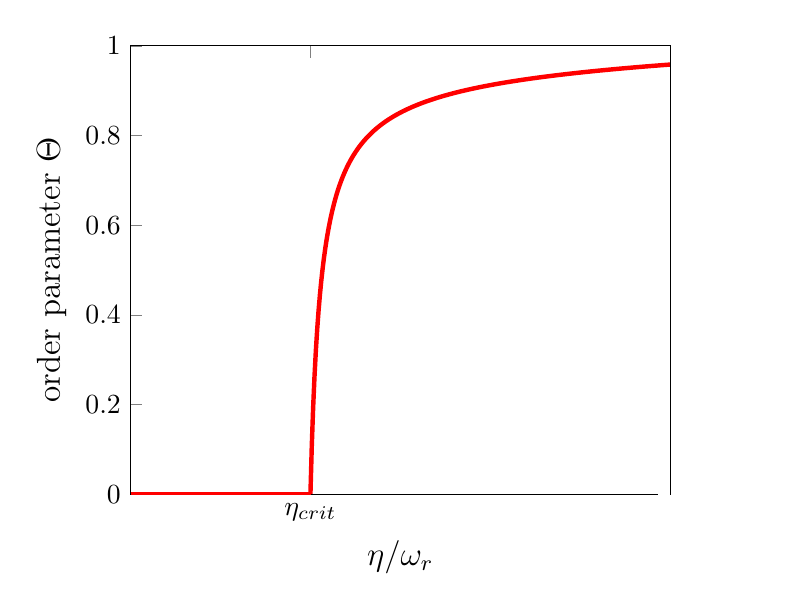
\begin{tikzpicture}
\begin{axis}[
    %title={Temperature dependence of CuSO$_4\cdot$5H$_2$O solubility},
    ylabel={order parameter $\Theta$},
    xlabel={$\eta / \omega_\text{r}$},
    xmin=0, xmax=15,
    ymin=0, ymax=12,
    xtick={5},
    ytick={0, 2.4, 4.8, 7.2, 9.6, 12},
    xticklabels={$\eta_\text{crit}$},
    yticklabels={0, 0.2, 0.4, 0.6, 0.8, 1},
    %ticks=none,
    label style={font=\large},
    legend style={font=\small},
    legend pos=north east,
    ymajorgrids=false,
    grid style=dashed,
    every axis plot/.append style={ultra thick}
]
\addplot [
	restrict y to domain=0:12,
    domain=0:15, 
    samples=400, 
    color=red,
]
{(x+0.279663-5)^(1/4) - 3/(x+0.279663-5) + 10};
\addplot [
	%restrict y to domain=0.2:3,
    domain=0:5, 
    samples=400, 
    color=red,
]
{0};
\end{axis}

\begin{axis}[
  ymin=0, ymax=10,
  xmin=0, xmax=10,
  hide x axis,
  axis y line*=right,
  %ytick={2, 4, 6, 8, 10},
  %yticklabels={-4, -2, 0, 2, 4},
  ylabel={ylabel},
  ylabel near ticks,
  ylabel style=white,
  yticklabel style=white,
  ytick style=white,
]
\end{axis}
\end{tikzpicture}
\end{document}